\documentclass[aps,prb,floatfix,twocolumn,twoside,english]{revtex4-1}

\usepackage[dvips]{graphicx}
\usepackage[latin1]{inputenc}
\usepackage{pstricks,pst-node,pst-text,pst-3d}
\usepackage{amsmath}
\usepackage{verbatim}
\usepackage{epsfig}
\usepackage[T1]{fontenc}
\usepackage{babel}
\usepackage{enumitem}

\setdescription{font=\small,labelindent=1cm,noitemsep,leftmargin=1cm,labelwidth=8mm,rightmargin=0.5cm}


\begin{document}

\title{Undergraduate students' challenges with computational modeling of physics}

\author{Simen A. S\o rby}

\affiliation{Department of Physics, University of Oslo, N-0316 Oslo, Norway}

%\author{Carl Angell}

%\affiliation{Department of Physics, University of Oslo, N-0316 Oslo, Norway}

%\author{Morten Hjorth-Jensen}

%\affiliation{Department of Physics, University of Oslo, N-0316 Oslo, Norway}

\date{\today}


\begin{abstract}

In later years, computational perspectives have become essential parts in several of the University of Oslo's natural science studies. In this paper I discuss some main findings from a qualitative study of the computational perspectives' impact on the students' work with their first course in physics -- mechanics -- and their learning and meaning making of its contents. Discussions relating to the students' learning of physics are based on the sociocultural theory, which originates in Vygotsky and Bakhtin, and subsequent physics didactics research. Results imply that the computational assignments' greatest challenge is their combined use of students' knowledge from earlier separated contexts. Making use of informatics, numerical and analytical mathematics and conceptual understanding of physics in one big package, appears as a clear challenge for the students. A lack of awareness considering the limitations of physical modeling is also observed. I argue in favor of helping the students create an awareness concerning their use of sufficient knowledge and system of conception, or ``tool set'', for the different tasks at hand. They need help creating a plan for their modeling and to become aware of its limits. In light of this, I propose a specific and dialogic text as grounds for the exercises, in which stress is laid on clarification and elaboration, to be of potential great aid for the students.

\end{abstract}

\maketitle

\section{Introduction}

Both computers and the great span in numerical methods for mathematical computations have gradually evolved due to scientific research with its endless stream of new questions and technology's seemingly unstoppable advancements. This development has in turn caused significant changes in a physicists expected tasks in his or her working life, be it either research or industry. As a consequence, computational perspectives have become essential parts in several of the University of Oslo's natural science studies, including the Physics, Astronomy and Meteorology branch, which is the subject of this paper. These changes are the results of some enthusiastic people working with a project called Computers in Science Education (CSE) at the University of Oslo.\cite{CMA_CSE} The goal of this project is to develop a unified computational perspective on undergraduate teaching programmes across course and departmental boundaries.

The students will in their first semester at the University gain important insight in analytical and numerical mathematics, as well as the programming language Python. The knowledge and skills they build up during this semester is fundamental for working with courses further up in the system. For the physics students in particular, the first semester will lay the foundation for modeling physical systems and phenomena with computational perspectives in their second semester and their first course in physics: mechanics. Computational perspectives are integral parts of this course and stands side by side with traditional physics theory. To accomplish this, new course materials have been developed -- including textbook material and exercises -- which incorporates these new aspects as a natural part of the curriculum. These new exercises involve writing program codes in python to simulate a broad range of physical systems on the computer. Since the CSE-project has truly started to bear fruits, it has been made possible to carry out a study on how these new aspects impacts the students work with and learning of physics. Some results from this study will be discussed in this paper. [more on motivating the reader?]


\section{Solving ordinary differential equations with Euler's Method}

Solving ordinary differential equations is often an essential part of working with physical systems. In this section, I will first show how the general mathematics makes it's way to the program code for simulating a physical system. In the end of the section, I will outline the assignments the students in this study were set to do. 

So without delay, let's introduce the general second order ordinary differential equation (ODE):
\begin{equation}
x''(t) + P(t)x'(t) + Q(t)x(t) = 0 \nonumber
\end{equation}
\noindent Or written in a slightly different fashion:
\begin{equation}
\label{eq:andreordensdiff}
x''(t) = f(t,x(t),x'(t))
\end{equation}
\noindent The first step in solving this equation, is to introduce a new variable, $y(t)$, with the relation $y(t) = x'(t)$. Instead of solving the second order ODE in equation \ref{eq:andreordensdiff}, we can now solve the two coupled \textit{first order} ODE's in equations \ref{eq:set_ode1} and \ref{eq:set_ode2}:
\begin{subequations}
\begin{align}
 y'(t) &= f(t,x(t),y(t)) \label{eq:set_ode1}\\
 x'(t) &= y(t) \label{eq:set_ode2}
\end{align}
\end{subequations} 
\noindent A method for approximating a general first order ODE's, $y'(t) = f(t,y(t))$, can be derived from the definition of the derivative:
\begin{equation}
 y'(t) = \lim_{\Delta t \rightarrow 0} \frac{y(t+\Delta t) - y(t)}{\Delta t} \nonumber
\end{equation}
\noindent By changing $\Delta t$ into a discrete value, $h$, we get Euler's method:
\begin{align}
 y(t+h) &= y(t) + y'(t) \cdot h \nonumber \\
	&= y(t) + f(t,y(t)) \cdot h \nonumber
\end{align}

Euler's method is an iterative numerical method which is applied to arrays of discrete values, in which $h$ becomes the step length between each value. Using Euler's method on equations \ref{eq:set_ode1} and \ref{eq:set_ode2}, with regards to the $i$'th element in the arrays, gives us:
\begin{subequations}
\begin{align}
  y_{i+1} &= y_i + f(t_i,x_i,y_i) \cdot h \label{eq:euler1} \\
  x_{i+1} &= x_i + y_i \cdot h \label{eq:euler2}
\end{align}
\end{subequations}
\noindent If we are able to set initial conditions ($x_0$, $y_0$ and $t_0$) for the system, approximated solutions for \ref{eq:set_ode1} and \ref{eq:set_ode2} may be iterated with \ref{eq:euler1} and \ref{eq:euler2}.

A typical physics problem in mechanics can be described with Newton's 2. law, $\sum{F} = ma$. This equation is equivalent to that of equation \ref{eq:andreordensdiff}:
\begin{equation}
\label{eq:newton}
a(t) = x''(t) = \frac{1}{m} \sum F(t,x(t),v(t)) \nonumber
\end{equation}
\noindent In this case, we introduce the variable $v(t)$ with the relation $v(t) = x'(t)$ and get the following set of equations.
\begin{subequations}
\begin{align}
 v'(t) &= \frac{1}{m} \sum F(t,x(t),v(t)) \nonumber\\
 x'(t) &= v(t) \nonumber
\end{align}
\end{subequations} 
\noindent After declaring constants, arrays (with length $n$) and initial conditions, the essential code for computing the approximated solution can be seen below. Here, as we run through the arrays, the sum of forces divided by mass is calculated in advance (and recognized as $a$) to ease readability. Also, the more common notation of $dt$ is used for the step length. The elapsed time is updated in the end of each step.

\begin{small}
\begin{verbatim}
   for i in range (n-1):
       a[i] = F(t[i],x[i],v[i])/m
       v[i+1] = v[i] + a[i] * dt
       x[i+1] = x[i] + v[i] * dt
       t[i+1] = t[i] + dt
\end{verbatim}
\end{small}

\noindent All physical systems that can be described with a second order ODE, can be approximated with this method. The only variables that differs from system to system is the forces in play, and consequently the only basic difference from code to code is the function containing these forces.

\subsubsection{Modeling a 100m sprint}
The first student assignment for this study considers a 100 meter sprint. The goal of this assignment is to go from a simple model to a more complex model and show how easily this is done from a computational perspective. The students start out by regarding the sprint with a constant drive force $F_D = 400 N$ and will show analytically the sprinters time crossing the 100 meter mark (which will, by far, be a new world record). To make the model more realistic, a more complex term is then added, namely a model for the air resistance, $D = \frac{1}{2}\rho C_D A(v-w)^2$. Here we have introduced some factors: the density of air, $\rho$; the cross-sectional area of the runner, $A$; the drag coefficient, $C_D$; and the velocity of the air (wind speed), $w$. Then, a program that determines the motion of the runner should be written. Hereafter, more terms are added for making the model even more realistic, namely a ``crouched phase'' in the beginning of the race, $f_c$, and a physiological limit of the runner, $f_v$, both with exponential dampening factors. In the end, the total driving force adds up to
\[
F = F_D + f_c e^{-(\frac{t}{t_c})^2} - f_v v - D \nonumber
\]
\noindent where 
\[
D = \frac{1}{2}(1-\frac{1}{4}e^{-(\frac{t}{t_c})^2})\rho C_D A(v-w)^2 \nonumber
\]
\noindent The only complications in the program code as a consequence of this is to keep the function for the acceleration written correctly.

\subsubsection{Ball in a spring}
The second student assignment for this study considers a ball with mass $m$ in a spring, or, as the exercise text says, a pendulum consisting of a ball in a rope moving in a vertical plane. In other words: An elastic pendulum motion. The force on the rope is described with a spring model with spring constant $k$ and equilibrium length $L$. The assignment starts out with asking the students to draw a free-body diagram and show that the forces in play can be written as
\begin{equation}
 \sum \vec F = -mg \hat j - k(r-L) \frac{\vec r}{r} \nonumber
\end{equation}
\noindent where $\vec r$ determines the position of the ball and $g$ is the gravitational acceleration.

Some more traditional exercises are given, like calculating analytically what the position will be if the velocity is zero, before a program code to describe the motion of the ball is asked for. The challenge here is to decompose the forces correctly and to implement this into the program code. Afterwards, some experimenting with the spring constant, $k$, is done, and limitations to this modeling approach is asked for.

\subsubsection{Kirkwood gaps}
The third student assignment of this study considers the system Sun---Jupiter---Asteroid, where the Sun is assumed to be stationary. Only the boys did this assignment as some mishaps arose when handing out the assignments this particular week (the wrong assignment was given to the girls, see below). In this assignment, most of the program code is given to the students for them to experiment with. Before this, however, they are asked for some analytical calculations on the forces in play and rewriting them with dimensionless variables. For the record, the forces in play for Jupiter and the asteroid respectively, are 
\begin{align}
 \vec F_J &= m_J \vec a_J = -G \frac{Mm_J}{r_J^3} \vec r_J - G \frac{m_Am_J}{\Delta r^3} \Delta \vec r \nonumber \\
 \vec F_A &= m_A \vec a_A = -G \frac{Mm_A}{r_A^3} \vec r_A + G \frac{m_Am_J}{\Delta r^3} \Delta \vec r \nonumber
\end{align}
\noindent where $\Delta \vec r = \vec r_J - \vec r_A$. The sun has mass $M$ and is set to be in origo, where as $m_J$, $r_J$, $m_A$ and $r_A$ are the masses and positions of Jupiter and the Asteroid respectively. $G$ is the gravitational constant.

One of the interesting parts for this paper in particular, is an exercise where the students are asked to experiment with the initial conditions for the velocity and mass. We will return to this event in the results section of this paper.

\subsubsection{Dynamics of a periodically driven pendulum}
This assignment was done only by the girls, as it was given to them by a mishap (they were not meant to solve it). Some interesting discussions arose nevertheless, so I'll give a quick description of the assignment. As with the boys' assignment, big parts of the program code is given in this assignment as well. In this case, we consider a thin stiff rod of length $L$ with a small sphere in the end with mass $m$. A simple model for the sphere's air resistance is also included, namely $F_f = -qv$, where $q$ is a constant and $v$ is the sphere's speed. In addition, the pendulum is also subject to a periodically varying torque around the attachment point, $\tau_z = \tau_{z0}\sin(\omega_z t)$, where $\tau_{z0}$ and $\omega_z$ are constants. The first thing the students are set to do, is to draw a free-body diagram and show that the differential equation for the motion can be written as:
\begin{align}
 \tau(\theta,t) &= -mgL\sin\theta - qL^2 \frac{d\theta}{dt} + \tau_{z0}\sin(\omega_z t)\nonumber \\
		&= mL^2\frac{d^2\theta}{dt^2}\nonumber
\end{align}
The challenge here is mainly keeping in mind all mathematical relations for coordinate changes and recognizing $\frac{d^2\theta}{dt^2}$ and $\frac{d\theta}{dt}$ as the angular acceleration and velocity respectively.

\section{Theoretical framework}

\subsection{The sociocultural theory of learning and development}

The sociocultural theory of learning emphasize that knowledge is constructed through social interaction and in a specific context, not primarily through individual processes. Knowledge is consequently situated in a historical and cultural context. The construction of knowledge involves mediation of concepts on a social plane, which can thereby be internalized by the individual.\cite{Wertsch:1985} Lev Vygotsky is widely recognized for introducing these ideas along with, what he calls, the Zone of Proximal Development (ZPD) in school children's learning and development.\cite{Vygotsky:1978} The ZPD, as defined by Vygotsky himself, \textit{is the distance between the actual development level as determined by independent problem solving and the level of potential development as determined through problem solving under adult guidance or in collaboration with more capable peers}. With guidance and collaboration being viewed as essential for learning and development, the act of imitation should as a consequence be regarded as an active process in which meaning and understanding is being constructed. When imitating someone else, the student finds himself within his ZPD on his way of mastering the task at hand on his own.

Regarding the social mediation of concepts, Vygotsky made a clear distinction between two types: \textit{spontaneous} and \textit{scientific}.\cite{Vygotsky:1986} Spontaneous concepts are characterized by having grounds in everyday experience and being unsystematic and strongly bound to context. Scientific concepts, on the other hand, are decontextualized and organized in a logic and hierarchic fashion. The latter are also called ``academic concepts'', i.e. concepts found in any school setting. Even though spontaneous and scientific concepts are fundamentally different in the way we encounter and learn them, they are closely related to each other in the development of concept formation: Spontaneous concepts have a development direction ``upward'' towards greater abstractness and, at the same time, they arrange for establishing scientific concepts in their ``downward'' development toward greater concreteness. The challenge teachers face is to hinder the spontaneous concepts from being overly bound to specific contexts, and at the same time hinder the scientific concepts from appearing isolated and fragmented.

When we now turn to the works of Mikhail Bakhtin, we'll take a deeper dive into \textit{how} the social mediation of concepts might take place. The main means for this process is oral or written discourse. Bakhtin pointed out that any discourse, or interplay of \textit{voices}, consists of addressed \textit{utterances} which are composed with grounds in a \textit{social language}.\cite{Wertsch:1991} A social language can be viewed as the basis of values and knowledge for the composition of the utterance; a specific point of view determined by one's social position, e.g. one's profession or other social affiliation. On the other hand, what Bakhtin refers to as ``voice'' should be compared with one's personality or consciousness. One's voice exists fundamentally in a social milieu and cannot be isolated from other voices. This applies for the utterance as well, however it is also being \textit{addressed}; it carries a natural expectance of a response. This can very well be an expectance of no response at all. In such a case, the utterance is regarded as \textit{authoritative}. An authoritative utterance implies that it's meaning is static, it is fixed once and for all and does not encourage an interanimation of voices. The opposite of an authoritative utterance is a \textit{dialogic} utterance. In this case, the meaning is not fixed and static, but open -- it seeks new contexts to broaden its meaning. The number of such contexts are limited by the number of and heterogeneity of the voices that has the opportunity to participate in the discourse. The more contexts one can relate to a concept, or the more associations one can make, the easier it's meaning might be to grasp.\cite{Kubli:2005} To be meaningful or of a meaning making character, the discourse should contain multiple voices which engage each other dialogically; it should strive for multivoicedness, or \textit{polyphony}, and be dialogic in nature.

Mortimer \& Scott follows the lead of Jon Ogborn and colleagues and compare, with grounds in Vygotskys view on concept formation, learning of a school subject with \textit{building up its scientific story}.\cite{Mortimer:2003,Ogborn:1996} With regards to Bakhtin, the scientific story of physics is regarded as the physics theory expressed in terms of the ideas and conventions of the school science social language. Teaching of physics then becomes the equivalent of ``telling'' the story in its social language in a convincing way for the student, i.e. engaging the students everyday views in a topic area and developing convincing lines of argument through an interactive and dialogic dialogue. The latter is fairly important to bear in mind: A dialogue, or any discourse, may very well be interactive without being dialogic -- it depends on whether it opens for an interanimation of voices or not. If the other's voice isn't \textit{heard} (i.e. taken into account), the discourse is not dialogic.


\subsection{A conceptual understanding of physics}

A much discussed phenomenon is how the students are able to solve assignments and doing well in tests without being able to show the ``correct understanding'' of the physics theory. It may vary from not being able to show \textit{any} understanding, to showing a faulty understanding from a scientific point of view. While the first case is the result of rote memorization, the latter, often labeled as common sense concepts or \textit{misconceptions}, is the results of the students' having developed an individual (and faulty) understanding of the physics theory, often combined with memorization. The problem with misconceptions is that they are not arbitrary mistakes; they are firmly ingrained in the students' understanding of the concept.\cite{Hestenes:1985,Gautreau:1997} They are the tools for the students' everyday language and acts to define their way of talking and thinking.\cite{Mortimer:2003} 

Instead of labeling all such faulty understanding as misconceptions, Angell proposes to rather view them as \textit{alternative conceptions} or \textit{intuitive ideas} which might contain some degree of consistency and correct understanding.\cite{Angell:2004} Portions of the students understanding should be regarded as \textit{fragmented knowledge} which needs to be developed and refined into a more systematic scientific understanding.

When the students aren't holding the ``correct understanding'', it is common to label it as having an erroneous \textit{conceptual understanding} (might need citations?). With grounds in the previous section, a conceptual understanding involves being able to tell and understand a subject's scientific story in its social language. Understanding of this story involves grasping it's scientific concepts and relating them to fruitful spontaneous concepts and other scientific concepts which acts explanatory to the story being told. Showing conceptual understanding involves therefore expressing it with words. Henriksen and Angell even propose that ``to think like a physicist is to talk like a physicist''.\cite{Henriksen:2010}

Several ways of dealing with misconceptions in teaching have been proposed, one being Peer Instruction.\cite{Mazur:1997} This method has been incorporated into the teaching of the students' mechanics course at the University of Oslo and involves conceptual questions with several answers being presented to the students during lectures. Importantly, only one answer is correct, while the others can contain more or less regular misconceptions. The main thought is that the students gain valuable insight by discussing the different answers with their neighboring students or with the lecturer. 

[Related to this matter, students' reported gain in tests after watching different kind of multimedia treatments, clearly favors discussions which deals with misconceptions through dialogic discourse.\cite{Muller:2008}]


\subsection{Traditional and computational modeling of physics}

Describing natural phenomena with mathematics is traditionally what physics is all about. Mathematical models can be made, for instance, for describing and predicating complex phenomena in the most precise fashion (like meteorologists do), or for studying the fundamental behavior of a phenomenon when having ``peeled off'' most of the complications nature puts on it (like some theoretical physicists do). 

Models can be regarded as bridges between the scientific theory and the world as experienced; they can be a helpful tool for visualizing and concretize abstract phenomena. They can also help the school subject becoming more authentic, giving insight into the way scientists do their work and the creativity that underlies the nature of scientific progress.\cite{Gilbert:2004}

Traditional modeling of physics does, however, not only require knowledge in analytical mathematics. Angell points out that students working with empirical-mathematical modeling in school has to deal with several \textit{representations} of the physical phenomenon.\cite{Angell:2008} As an example, the phenomenon ``free fall'' may be viewed with an experimental, graphical, pictorial, conceptual and a mathematical representation.

Computational modeling of physics involves even more aspects than traditional modeling. While working with computational modeling, the students still have to regard an analytical mathematical model of the physical system, but in addition, they have to develop an algorithm for solving the assignments on their computer. For doing this, they have to make use of knowledge in numerical mathematics and programming for experimenting with their physical system, exploring ideas and assessing results. 

Futschek gives some thoughts on what he calls ``algorithmic thinking'' -- that is, the pool of abilities needed for constructing an algorithm in an adequate manner. This involves abilities in analyzing a given problem, specifying the problem precisely and finding the basic actions needed to construct the algorithm for the problem at hand.\cite{Futschek:2006} Landau describes his views on ``computational scientific thinking'' as the ability to use one's knowledge of theory, model, method and implementation to assess, visualize and explore a physical system with the means of experiments and simulations.\cite{Landau:2006} (more citations from Landaus work, perhaps?) Sins and colleagues gives some thoughts on what teachers should keep in mind under novice students' computer based modeling (in this case with a drag-and-drop based program called PowerSim).\cite{Sins:2005} They point out, among other things, that the modeling should include \textit{(sub)goals} for helping the students more easily grasp how the model structure affects the behavior of the phenomenon at hand. They also observe how the less skilled students often resort to a \textit{model fitting behavior} in which stress is laid on tuning model parameters in hope of getting an output resembling the observed empirical data instead of discussing more deeply the model's elements or structure.


\section{Methods}

Questions regarding learning and meaning making of physics require methodological aid from the social sciences. This study revolves heavily around qualitative observations of two pairs of students solving compulsory assignments in mechanics. Three assignments with a considerable degree of computational perspectives were chosen to give grounds for the observations. Qualitative observations was primarily chosen for gathering data as it seemed like the most obvious way of gaining valuable insight into \textit{how} the students' work with the computational aspects might go on and what challenges they might face. Something more ...

Also: Make sure to point out that all transcribed discussion in this paper have been translated from Norwegian -- and double check with a fair amount of people that the translations transfer the same meaning.




\section{Results and discussion}


\subsection{Working in modes}
\label{sec:modes}

One of the first observations made, was the students' tendency to find themselves in ``working modes''. Depending on the exercise at hand, the students' work tended towards either conceptual knowledge of physics and everyday experience (``physics mode''), mathematical relations and arithmetic calculations (``math mode'') or sheer programming techniques or the programming language's syntax (``programming mode''). The physics mode and math mode has been documented by others,\cite{Angell:2008} and were essentially the source of inspiration for trying to document these modes myself. The ``programming mode'', however, is a result of the new computational perspectives introduced in the mechanics course and consequently a brand new mode. As well as the characterizations mentioned above, the programming mode have some other features as well. When writing program codes, the students' work has very little structure and they seem to enter some sort of ``trial and error''-mentality for handling even the most basic problems, be it either mathematical, physical or computer based (i.e. programming techniques or language syntax) in nature.

First, I'll illustrate the physics mode. The two boys are about to draw a free-body diagram of a sprinter running a 100-meter sprint:

\begin{description}
\small
\item[] \textit{The physics mode:}
\item[G1] Should we not just -- isn't a free-body diagram just -- like this?
\item[G2] Yes, but look -- at the start, he'll have a kind of log [starting blocks] to lean against and...
\item[G1] Nobody has said that.
\end{description}

G1 is correct. Nobody has said that; the model has no such condition (yet). Even so, G2's initial thoughts are set on the real race -- his first analysis of the race is based on spontaneous concepts originating from everyday experience (e.g. running himself, watching sprints on the television, etc.).

Second, a bit later in the same assignment, the boys are reluctant to seek aid from course material and want to solve the exercise ``Write a program to determine the motion of the runner from start to the finishing line'' on their own:

\begin{description}
\small
\item[] \textit{The math mode:}
\item[G2] No, but we have... We have an expression for the double derivative with the first derivative. And then we have the position as well -- we have $x$ -- hmm. We have, like, no... It's been a long time since I've done this.
\item[G1] But...
\item[G2] Like, we have a system of differential equations $x_1^{\prime} = x_2$. 
\item[G1] M-hmm? 
\item[G2] So we'll get out values for $x_1^{\prime}$ and $x_2^{\prime}$ -- or the velocity, that is.
\item[G1] What's that?
\item[G2] If we solve this, we'll get values for $a$ and values for $v$. And we can use Euler's, can't we?
\item[G1] Yeah, we can just use Euler to solve those two and you'll integrate that, then -- what'll you get -- then you'll get your velocity?
\item[] [... some time is being spent on looking through the course material by my suggestion, but G1 won't settle with such an easy solution ...] 
\item[G1] No, I don't understand why this should be so difficult. Isn't this just a completely standard Euler? Where we can choose a standard Euler and we have a function $f(v,t)$? Which gives a...
\item[G2] Yes, wait a minute!
\item[G1] Then we'll get, like...
\item[G2] A standard Euler? $x_{i+1} = ...$ or should we look at the speed as well?
\item[G1] $v_{i+1} = a_i dt$ where $a_i$ is always [... reads the expression for the acceleration ...] and we've got $v_0$. There's nothing stopping us?
\end{description}

The recalling of different fragments from the previous semester's course in numerical mathematics, gives this discussion a clear math mode-characteristic. Instead of talking about velocities and accelerations, G2 tends to call them ``$x_1^{\prime}$ and $x_2^{\prime}$'', and instead of saying ``$a(v,t)$'', G1 uses the more mathematical ``$f(v,t)$'', all the time focusing on the mathematical relations. Nevertheless, in the end they're able to bring their discussion over into a physics context -- the scientific, abstract mathematics are being related to something specific and definite. The fundamental mathematics, however, is being recalled from a distinct mathematical context; the students initially find themselves in math mode.

Finally, we'll have a look at the programming mode. As a first example, the two girls are working with modeling a 100-meter sprint. They have ended up with different values for the starting acceleration and have already spent some time going over J2's program code looking for typical syntax errors. They now discuss, rather shallow and while sitting in front of their respective computers, which value of the starting acceleration seems most plausible:

\begin{description}
\small
\item[] \textit{A starting acceleration of either 5,5 m/s$^2$ or ...:}
\item[J2] I think it's a bit hard to say if it's reasonable, that he can have 11 m/s$^2$ in the beginning as acceleration! Well, that's absurdly high!
\item[J1] No, well, I don't think it's reasonable!
\item[J2] No, but I'm just thinking about it declining so fast.
\item[J1] Yeah, but well... Either it's something wrong with my program, or it's something wrong with your program, 'cause we should have the same. And I regard my acceleration as more plausible than yours! *Laughs*
\end{description}

J1 opts for comparing the codes one more time. To solve this problem, the easiest solution seems to be looking for faulty lines of code. She also somewhat sets the mode to trial-and-error by means of comparison. 

Another example takes place in the girls' third assignment. They have been given a working program code, with the exceptions of some values which have to be filled in. In this code, the angular acceleration is not stored in an array, something both girls believes it has to be. If not stored in an array, it would be constant, they seem to think:

\begin{description}
\item[] \textit{The need of an array?}
\small
\item[I] Do you need an array for alpha?
\item[J2] Yes.
\item[J1] Hmmm...
\item[I] Why is that?
\item[J1]  You probably don't need to store it all the time, but... It's not constant. I think. I don't know. We can try something clever, we can try writing it like this, then we can see if it behaves like it's constant.
\item[] [...]
\item[J2] But in the way he has written it, it looks like alpha is a constant.
\item[] [...]
\item[J1] Like he has written the program? Yeah.
\item[I] Why is that? 
\item[J2] He hasn't written any index, ``holdt jeg p� � si''?
\item[J1] Because he hasn't given any alpha\_0 and no array for alpha or anything. But it could be something we should find out by ourselves.
\item[I] But the way you have written alpha right there. If you don't store it as an array, would it still be constant for every loop?
\item[J1] Since you're asking, it probably won't! But I think it should be!
\item[I] Yes, I'm probably giving some hints right now.
\item[J1] Oh no, yeah, so you'll just update it every time -- yes, that's clever!
\end{description}


The girls should not need to ``try writing it like this'' and then ``see if it behaves like it's constant'' -- a clear trial-and-error solution. At the same time, their mind is set on the visual syntax of the program code, not on Euler's method and how it behaves. They focus on how the code has usually been written in similar contexts, not so much on the problem at hand.

Lastly, the boys are writing a program for the elastic pendulum:

\begin{description}
\small
\item[G1] Do you make unit vectors, or what?
\item[G2] Hmm? 
\item[G1] [Makes a decision without getting a response:] No, I'll just make these vectors and hope that Python is able to multiply them on its own.
\end{description}

Here, G1 lets Python determine if what he thinks should work, actually works or not. He doesn't need to know on beforehand if it is going to work -- he rather trials and hopes for no errors. Furthermore:

\begin{description}
\small
\item[G1] I feel like this is kind of sketchy. From my part.
\item[G2] Yeah, I too feel it being kind of sketchy, because -- that $r$ -- that's... 
\item[G1] Yes, I have to make an $r_0$ and a $v_0$, thank you. 
\item[I] What is it that's being sketchy at the moment?
\item[G1] No, I just... I'm not entirely certain of what I'm doing. So I'll rather just gradually see if I'm doing something wrong.
\end{description}

The programming lacks structure and relies to a great extent on a trial-and-error mentality along with recalling of similar tasks from earlier programming contexts. The students seem to be in need of some sort of plan and be made aware on what they \textit{should} do -- not just what they \textit{may try} to do.


\subsection{Starting to program without having a plan}

As mentioned in the previous section, the programming mode seems to lack ``a plan'' on how to create the program and how the programming should go forth. This may not seem so strange when they, in fact, never makes one. The students never opt for analyzing given problems or specifying them precisely. Instead of giving examples of this, I'll rather illustrate the one exception. Here, G2 makes an attempt to create a plan, but encounters heavy resistance: 

\begin{description}
\small
\item[G1] But, are we still supposed to do this analytically?
\item[G2] Nope! 
\item[G1] No, that's what I was about to say. I propose that we rather... [rolls towards the computers] Well, he haven't said anything about it, so we may do this however we want to?
\item[G2] The $m$ was...? Eighty. Then we should solve the system? [continues with pen and paper]
\item[G1] Yeah, but it doesn't say that we're supposed to do this analytically?
\item[G2] ``Write a program to determine the motion''. 
\item[G1] Yes, we can use the program to find the $v$ for us.
\item[G2] We still have to find out which equations we should put into the program. He doesn't ask about the acceleration.
\item[G1] No, but we'll integrate with the computer?
\item[G2] Yes! But first we have to... We've got an expression for the acceleration dependent of the velocity. And then we're supposed to find the position, that is $x$, so we have to integrate $a$ two times, right? It's dependent of the derivative of ... So it won't be an easy integral, in other words. I'm unable to explain it, but ...
\item[G1] No, I understand what you're saying, but ...
\end{description}

As the assignment is to be done on the computer, it seems natural to the students to take a seat in front of the computer sooner rather than later. Possible problems needs not to be discussed, but met when they arise.

\subsection{The length of the discrete steps}

Since problems are met as they arise, the value of the step length or possible problems that it can cause are never discussed on beforehand. The few times the step length is mentioned, a discussion never gets started. Instead, it generally is set to its ``usual value'' of 0,1. In the following example, the boys are getting rubbish plots of an elastic pendulum motion. In their strive for solving this problem, G1 illustrates his view on the step length, $dt$:

\begin{description}
\small
\item[G1] That $r$ of mine is alarmingly similar to itself, ``holdt jeg p� � si''. Okay. There's something wrong with ... Ah, no wonder, ``$v + dt \cdot a$'', my $a$ must be erroneous.
\item[] [...]
\item[G2] Well, I think it's as early as my acceleration.
\item[G1] Ha-ha, that's what I'm thinking as well. Ah, this is weird. When I print out $r_0$ times -- this is $r_0$ -- and then I multiply it with $dt$, I get zero! 
\item[] [...]
\item[G1] So $v_1$ is correct. And $r_1$ is given by $r_0$, which is correct, plus the velocity $v_1$, which is correct, times $dt$.
\end{description}

Here, G1 has declared $dt$ as the total time divided by the number of steps, but since he has not made it explicitly a decimal number, it becomes an integer and therefore zero. The last sentence, however, is being uttered after this particular problem has been solved. The interesting thing is that G1 implies that everything is correct except the step length, $dt$. Even so, he is unable to call new attention to it. It's once again being viewed more or less as static. He is showing good insight into Euler's method, but is still unable to solve the problem. In this case, the step length has been declared with a too large value. The possible problems caused by a step length being too large is by no means unknown to the students. When the girls encounter a similar problem and eventually are able to solve it, J2 utters in frustration:

\begin{description}
\small
\item[J2] He could perhaps have given a small tip that we should make a fair amount of steps? So that people don't sit around and ...
\item[J1] No, no, no, they have taught us about this regarding Foreward-Euler for a long time -- this we should know!
\end{description}

J1 is correct. They should know about this, and they seem to do -- they just need to be made aware.



\subsection{Selecting the tools for solving the problem at hand: working with models ... or reality?}

Since the computational modeling includes a lot of different aspects to the physical system at hand, the students need to have some knowledge on all the different aspects, they need to have good modeling skills and they need to know when to use different tools and different sets of knowledge for the different tasks at hand. This is challenging and by no means obvious for the students. As a starter, we can have a look at the girls discussion when they're trying to grasp the meaning behind a plot like the one in figure \ref{fig:discrete_acceleration}:

\begin{figure}[htbp]
\begin{center}
 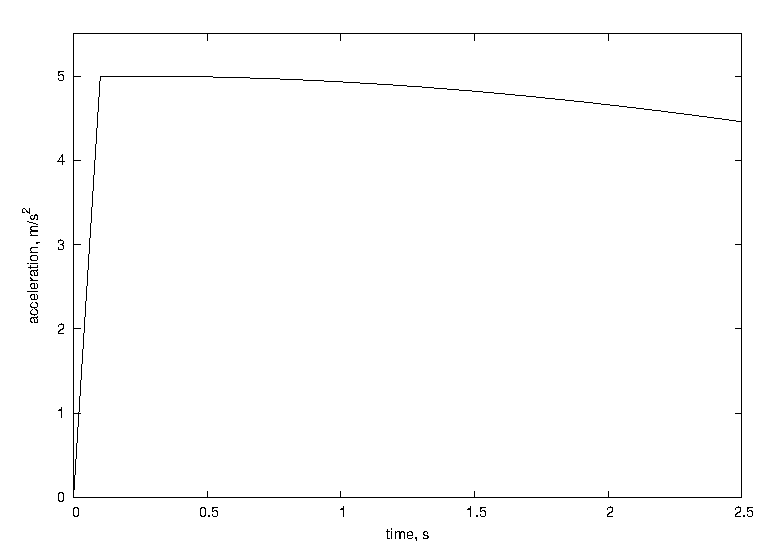
\includegraphics[scale=0.7]{figures/acceleration_error}
 \caption{An erroneous beginning of the sprinters acceleration due to discretization and a faulty line of code.}
 \label{fig:discrete_acceleration}
\end{center}
\end{figure}

\begin{description}
\small
\item[] \textit{The girls' discussion of a plot similar to figure \ref{fig:discrete_acceleration}:}
\item[J1] Do you get a somewhat weird beginning on the acceleration as well?
\item[J2] I don't know, I've messed things up a bit here right now, so ... On the acceleration? I don't know!
\item[I] What's a ``weird beginning''? 
\item[J2] A smooth start, perhaps? 
\item[J1] No, 'cause the acceleration starts at zero, but gets going very fast, so it becomes, like, straight up and such. And that's all natural compared to how he runs, but it just looked a bit weird. You would use a fraction of a second to get the acceleration from zero and up.
\item[J2] Yes? 
\item[J1] Yes, so it's all right.
\item[] [...]
\item[J2] I haven't gotten that, but ... 
\item[J1] That's why I'm asking, 'cause you haven't gotten that, but I have.
\item[J2] But it's very logical, isn't it?
\item[J1] I have no problem with it being like that. But I have in a sense no problem with it not being like that for you either, so I got a little -- ``what''?
\end{description}

The problem is in this case caused by setting the initial condition for the acceleration to zero, when at the same time calculation $a_{i+1}$ instead of $a_{i}$ in front of the steps iterating the approximated solutions. The graph's ``jump'' is merely caused by going from the initial value of zero to a calculated value in one time step. When looking at figure \ref{fig:discrete_acceleration}, it should ring a bell in the students' heads clinging ``discretization!'' Instead, they do not seem to know whether or not the plot makes sense. For J1, it does seem to make sense from an everyday point of view: The runner needs ``a fraction of a second to get the acceleration from zero and up''. When using her spontaneous concepts related to running she's able to make sense out of an erroneous graph.

Let's turn to the boys for our next example. Below, they are discussion a plot like the one in figure \ref{fig:Jupiter}:

\begin{figure}[htbp]
\begin{center}
 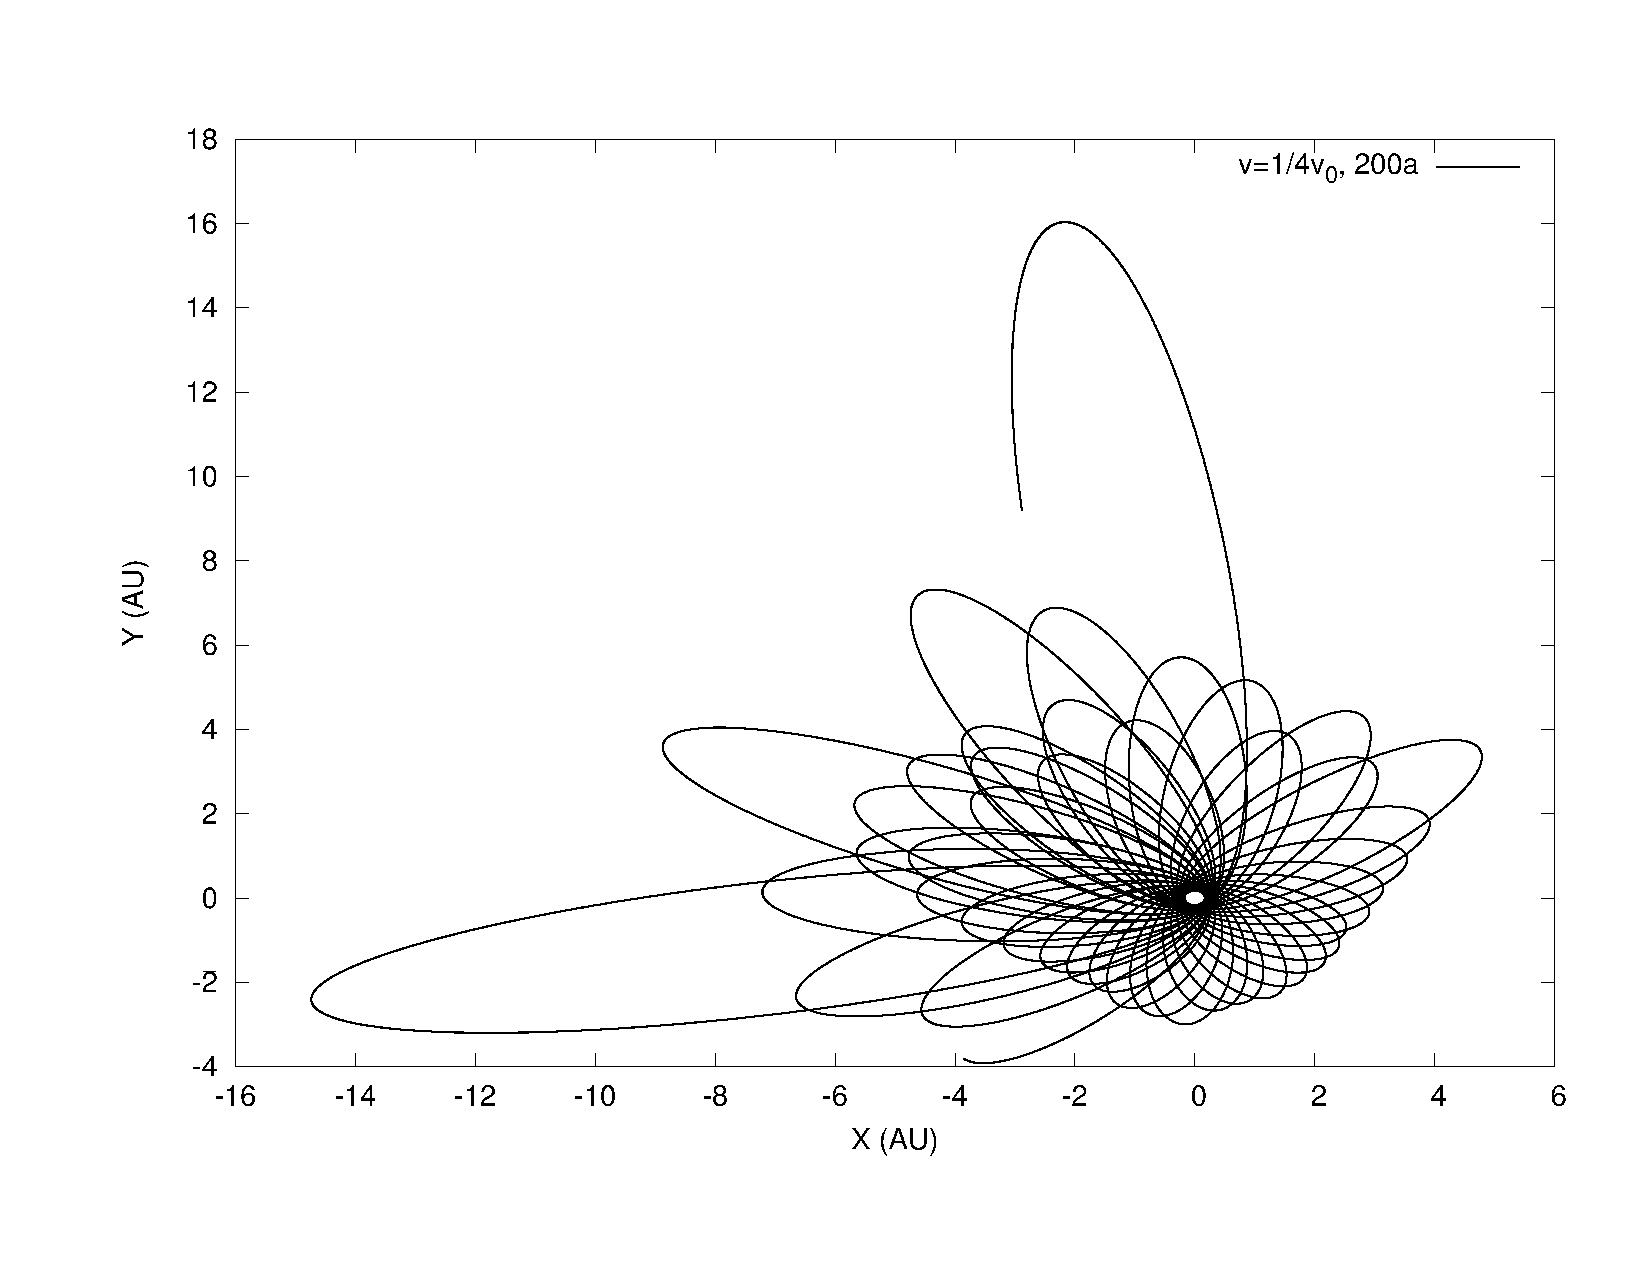
\includegraphics[scale=0.34]{figures/flower}
 \caption{The revolvement of Jupiter around the Sun at one fourth starting velocity ...?}
 \label{fig:Jupiter}
\end{center}
\end{figure}

\begin{description}
\small
\item[] \textit{The boys' discussion of a plot similar to figure \ref{fig:Jupiter}:}
\item[I] Do one fourth, like you did. [referring to G1's earlier attempt at one fourth starting velocity]
\item[G2] Nooooo, ok. Aiaiai!
\item[I] What happens here? 
\item[G2] Nah, it's hard to say. It gets sucked -- it starts there anyhow -- then it gets sucked in, and then it gets more and more energy?
\item[G1] Hmm? It can't get more and more energy?
\item[G2] But it bounces out to here!
\item[G1] Yeah, but at that point it's probably got zero velocity. 
\item[G2] Ah, right, I thought about it completely wrong. I'm tired today.
\item[G1] 'Cause it aaaalmost hits the Sun. Sweeps past the Sun. Or does it go through? No, it can't do that.
\item[G2] The program would have stopped.
\item[G1] Weeeell, would it?
\item[] [...]
\item[G2] No, I'm out of ideas. 
\item[G1] No, but what happens, there aren't really any errors happening here, is it? It's just that it's being sent abruptly out again after sweeping past the Sun? The Sun bends its path tremendously.
\end{description}

This discussion is somewhat similar to the girls discussion of figure \ref{fig:discrete_acceleration}. A lot of spontaneous concepts from everyday points of view are uttered in attempts to create meaning behind the plot, even though it's completely wrong. There is nothing in the model which would make the orbit change over time; it should stay an ellipse. Anyhow, as long as the Sun is able to bend Jupiter's path when it sweeps path the Sun at a close range, the plot makes sense for the boys. This is, however, not correct. The problem in this case is the step length being chosen to be too large. This causes a substantial numerical error arises when the curve bends abruptly.

In the last example, the boys are trying to simulate the elastic pendulum while, here as well, having chosen a step length being too large. They get a plot like the one in figure \ref{fig:rope}, and G2's spontaneous comments to this plot follows:

\begin{figure}[htbp]
\begin{center}
 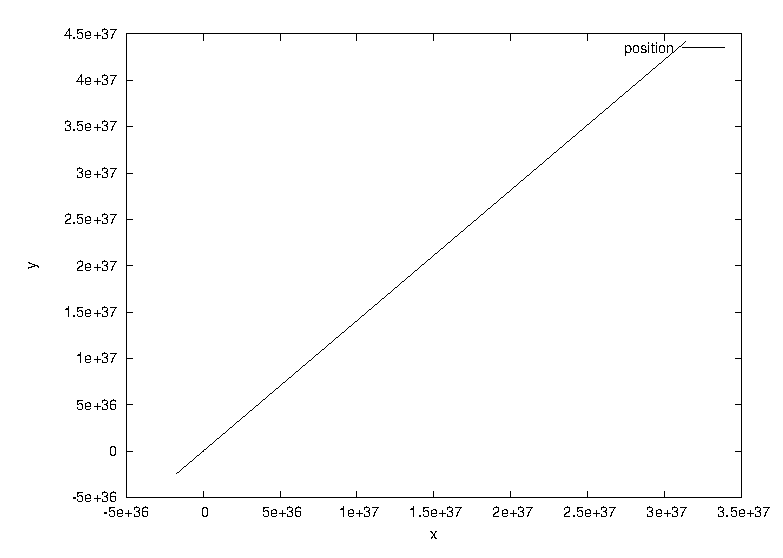
\includegraphics[scale=0.68]{figures/rope}
 \caption{Plotted position of the elastic pendulum with the step length being too large.}
 \label{fig:rope}
\end{center}
\end{figure}

\begin{description}
\small
\item[] \textit{G2's first thoughts on a plot similar to figure \ref{fig:rope}:}
\item[G2] Yeah, I would say that this position seems kinda doubtful. The pendulum just -- ``pjiuoooo'' [flies away].
\item[] [...]
\item[G2] I don't get this. It just dances upwards. Just like the spring being totally crazy.
\end{description}

A bit later, after having gotten some help by myself on solving the problem with the step length, the boys are trying to solve the exercise \textit{``Rerun the program with $k = 2000.0$. Describe the motion in this case. How can you use this method to model a pendulum in a stiff rope? What do you think would be the limitation of this approach?''} They quickly understand that a stiffer rope can be achieved by increasing the spring constant, $k$. Once again they get a plot like the one in figure \ref{fig:rope}. Even so, when trying to describe and explain what the odd behavior may be caused by, some noticeable comments emerge (from a rather long discussion):

\begin{description}
\small
\item[] \textit{Some comments to a plot similar to figure \ref{fig:rope}:}
\item[G2] It just implodes! It gets so large [...] I think in a way it gets so powerful it can't stay still without going bananas?
\item[][...]
\item[G1] It's like -- if you pull --- like... Can it get so big that if you pull it just slightly, it flies absurdly far away?
\item[G2] Yes? If a spring has the potential of exerting 40000 Newton if you pull it one micrometer, you can think what'll happen if it's L long.
\item[G1] Yeah, exactly!
\item[][...]
\item[G1] Like, see that you have a metal rod, and pulls it slightly, it will... Noooo, perhaps it does that as well.
\item[G2] If you pull a metal rod, you will deform it. It won't pull itself back together again.
\item[][...]
\item[G1] Yeah, but in this model... Does it exert a force if this is a rope and you pull it and let it go... A rope won't push the other way. A rope will just go up and... A rope just pulls, it doesn't push.
\item[G2] But if the rope has a $k$ of 40000, it will push.
\item[G1] What? No, what I mean is, a rope will only have a spring force if you pull, not if you push. If you push it in, it will only bend.
\end{description}

They use a great deal of time discussing springs going bananas, metal rods and ropes, but they never starts discussing \textit{the model} and the \textit{limitations of computational modeling}. Although G1 several times utters ``but in \textit{this} model ...'', he never seems able to go into the details of Euler's method's stepwise iteration or the problems caused by a step length being too large. When \textit{discussing} the physical model, ``reality'' -- or the slightly altered reality -- comes first. The problem with the boys' reasoning is that there's nobody in this model ``pulling'' the spring (other than gravity), and with regards to preservation of mechanical energy, the observed behavior is absurd.


\subsection{Meaning making -- dialogue, polyphony and the interplay of concepts}

The positive effects of a good interplay of concepts is already illustrated in section \ref{sec:modes} with the ``\textit{The math mode}''-discussion. In that specific case, the boys are recalling scientific concepts in numerical mathematics and, when mediating the concepts on a social plane, they help each other to recall other concepts and to establish these concepts in a physics context for the task at hand. This is typical for the boys' work with the exercises and acts constructive in their meaning making process: one mentions an abstract scientific concept and the other connects it to something specific and concrete.

The good effects of dialogic dialogues can be illustrated with the complete opposite: the negative effects of the authoritative dialogue. As an example, we should look at section \ref{sec:modes} and the discussion ``\textit{A starting acceleration of either 5,5 m/s$^2$ or ...}''. The full discussion is quite long, and starts out with myself asking the question ``who has the right answer?'', to which they answer:

\begin{description}
\small
\item[J2] I think you have the right answer.
\item[J1] I think I have the right answer as well because it's closer to the original acceleration. 'Cause, an acceleration of 11 is completely insane, isn't it?
\end{description}

From the beginning, J1 disregards J2's answer as being ``totally insane''. A bit later in this discussion, in the part recited in section \ref{sec:modes}, J1 still has a clear authoritative point of view, as she doesn't take J2's uttering of the graph ``falling so fast'' into account. This whole problem gets solved once I intervene and challenge J1 with a falling object-experiment. The comparison of the gravitational acceleration with their thoughts of what a sprinter could achieve, gives J2 the sufficient backing to oppose J1 and get them to actually calculate analytically the acceleration at $t=0$, not just comparing codes and talking about what's most ``natural''.

This last part functions as an example of the importance of polyphony and guidance as well. My voice, in this case in the role of a more capable peer, intervenes and socially mediates a meaningful reference which helps the discussion reach a conclusion. The same is the case with the discussion, also in section \ref{sec:modes}, on ``\textit{The need of an array?}'' Here, my critically charged questions are enough to get J1 to realize her mistake and come up with the correct answer; a more capable peer's indirect critique of one hypothesis is sufficient to make a new, correct one, emerge.


\section{Conclusion and implications}

(Temporarily just a sketch)

\subsection{The fragmentation of knowledge: On working in modes and being bound to context}

Different exercises opt for different set of skills. These skills are learnt in different sets of context, in which ``comment on the results'' might be bound to high school physics, while knowledge in programming and discrete mathematics -- which are necessary for discussing the model and modeling in detail -- are bound to the first semester at the University. Scientific concepts and spontaneous concepts should go hand in hand, not be either fragmented or overly bound to context respectively.

\subsection{The lack of awareness: Modeling with brand new set of tools}

On the different tool sets and creating an awareness on how to use them, as well as creating an awareness on the differences between model and reality (and the limitations computer based modeling causes, e.g. discrete models). The new set of tools (programming and numerical mathematics) needs to get actualized in a physics context. Discussing the model \textit{requires} insight into the numerical mathematics and programming, but, as with the boys' ``reality'', the next best thing to do is to make an ``inner consistent understanding'', even though it might be erroneous. Angell's representations and Landau's computational scientific thinking demands a lot of awareness on the different tools and skills.

The students' are able to ``model'' without discussing or showing modeling insight. They should be discussing the model and the modeling with their respective restraints on nature, or ``reality'', when they instead discuss the \textit{real} physical system. When ``comment on the results'' enter the picture, the students leave programming mode in favor of physics mode and starts discussing the physical system in an inadequate fashion. [They need to be pointed to how and what to comment!] Talking about physical systems has its context bound to high school physics, where numerical mathematics and programming were out of the picture. 


\subsection{Developing modeling skills by imitating ``the skilled modeler''}

On Futschek's algorithmic thinking and how one should ``make a plan'' and on Vygotsky's view on imitation and how the students should somehow be able to imitate ``the skilled modeler'' (one who has good modeling skills -- he makes a plan and is aware!).


\subsection{On building up ``the scientific story'' of physics}

On narrating (or ... \textit{telling}) the scientific story. Dialogue and room for alternative hypotheses and multiple points of view. Theory fragments needs to be elaborated and connected to each other for developing ``deeper insight''. Understanding why one thing is erroneous, contributes to understanding why the other is correct.


\subsection{The exercise text as the narrator of the scientific story}

I propose that the exercise text can be both a good narrator of the scientific story and the grounds for imitating good modeling skills. It demands, however, a certain amount of awareness concerning aspects of learning when constructing the text. The text should be both instructing as well as elaborating. It can help the students grasp the scientific story, rather than testing if they are able to narrate it on their own given the right amount of story fragments. Important: Dialogic and polyphonic in nature, to a certain extent.

\begin{acknowledgments}
Carl Angell, Morten Hjorth-Jensen and Anders Malthe-S�rensen.
\end{acknowledgments}


\bibliography{article_ref}


\end{document}

